\documentclass[final,letterpaper,twocolumn]{EIQ_UCR}

\titulo{Informe Parcial I}
\autor{Valeria Maya Roldán}
\autor{Sergio Manrique}
\autor{Maria del Mar Arbelaez}
\direccion{Universidad de Antioquia}
\curso{Informática II}
\fecha{21 Y 28 de Febrero, 2021}

\begin{document}

% Encabezado
\encabezado

% Cuerpo del artículo (No cambiar, me parece que tiene buena estructura)
\section{Introducción}
\label{sec:Introduccion}
%SE HACE AL FINAL
Introducción. (En los informes de laboratorio puede omitirse si se incluye como un breve párrafo inicial en el Marco Teórico.) Una referencia \citep{buckley1985design}.

\section{Marco teórico}
\label{sec:Marco}

	Escriba acá la introducción y el marco teórico o conceptual del trabajo. Cuando requiera separar un párrafo de otro deberá dejar una línea en blanco entre ambos párrafos, si solo genera un salto de línea se compilará como un solo párrafo.
  
	Para citar las fuentes bibliográficas existen dos comandos principales $\backslash$cite\{\} y $\backslash$citep\{\}, el primero es una cita textual de los autores mientras el segundo los muestra entre paréntesis. La diferencia está en que la cita textual indicará solo el año entre paréntesis, mientras que la segunda encerrará todo entre paréntesis y el año va separado por una coma.

Cuando requiera introducir una cita debe anotar entre los corchetes la clave de las entradas bibliográficas, separando por comas cuando debe citar más de una fuente, pero primero debe asegurarse de enlazar a la bibliografía el archivo de base de datos bibliográfica en formato BibTeX. Existen gestores de bibliografía como Zotero (\url{www.zotero.org}) que facilitan esta tarea y pueden enlazarse con facilidad en Overleaf.

Ejemplo de una cita textual \cite{buckley1985design} y de varias citas entre paréntesis \citep{buckley1985design}.

Para más detalles sobre manejo de bibliografía puede consultar la documentación relacionada.

\subsection{Ecuaciones}

Veamos cómo introducir ecuaciones enumeradas, en este caso tomaremos como ejemplo el número de Reynolds ($N_{Re} = \frac{\rho D V}{\mu}$) que podemos expresar como

\begin{equation}
	\label{ec:Reynolds}
	N_{Re} = \frac{\rho D V}{\mu}
\end{equation}
donde $D$ es el diámetro del ducto, $V$ la velocidad lineal del fluido, y $\rho$ y $\mu$ la densidad y la viscosidad del fluido respectivamente.

% La nomenclatura puede definirse en cualquier punto pero solo aparece en la sección Nomenclatura ordenada alfabéticamente
\nomenclature{$N_{Re}$}{Número de Reynolds, adim.}
\nomenclature{$\rho$}{Densidad, \si{kg/m^3}}
\nomenclature{$\mu$}{Viscosidad, \si{kg/(m\,s)}}   % El comando \, se introdujo para separar m s
\nomenclature{$D$}{Diámetro, m}
\nomenclature{$V$}{Velocidad, \si{m/s}}

\subsection{Figuras}
Las gráficas y figuras deben exportarse a alguno de los formatos válidos para luego introducirlos al documento. La figura \ref{fig:DistribNormal} es un ejemplo de una gráfica, en este caso el archivo se exportó a formato PDF.

\begin{figure}[h]   % Busque la documentación sobre las distintas opciones de posicionamiento
	\centering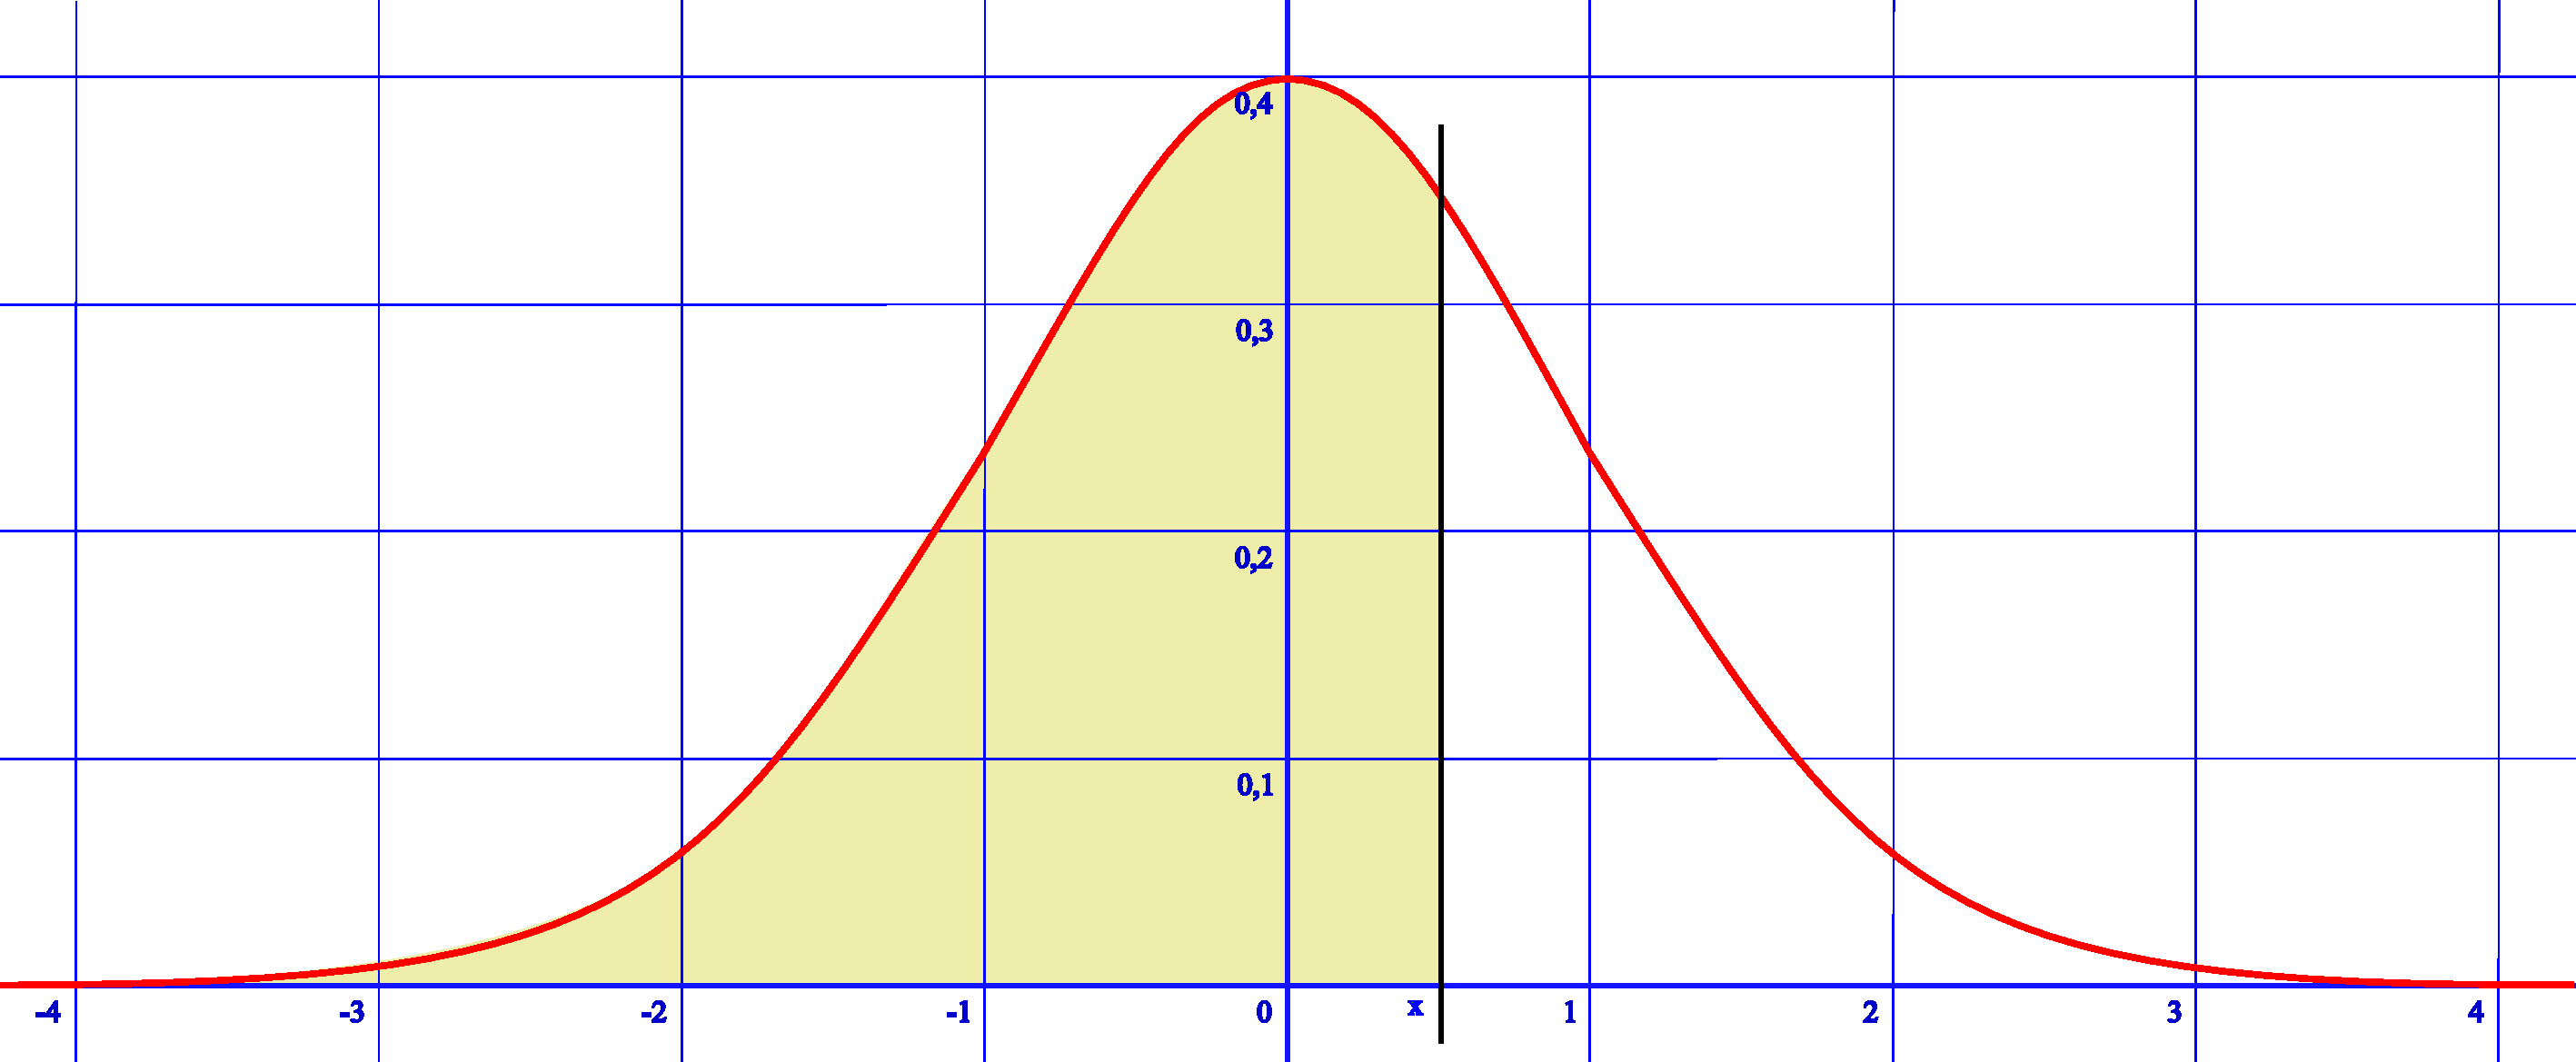
\includegraphics[width=1\linewidth]{Imagenes/DisNormal}
	\caption{Una gráfica de la distribución normal ocupando el ancho de una de las dos columnas del texto}
	\label{fig:DistribNormal}
\end{figure}

\subsection{Cuadros}
Generar cuadros en \LaTeX puede parecer complicado al inicio, afortunadamente eisten herramientas como \url{http://tablesgenerator.com/} que facilitan la labor, aun así debe comprenderse bien las opciones y darle un formato adecuado.

\begin{table}[h]
	\caption{Ejemplo de un cuadro con de propiedades}
	\label{Cuadro:Propiedades}
	\centering
	\begin{tabularx}{\columnwidth}{X X r}   % l: left, c: center, r: right
	\toprule
	Compuesto & $M$/(\si{g/mol}) & $T^{\circ}_{eb}$/(\si{\celsius}) \\
    \midrule
	\ce{H2O}  &   18.02    &   100     \\
	\ce{CO2}  &   44.01    &           \\
	\ce{H2SO4}&   98.079   &   337     \\
    \bottomrule
	\end{tabularx}
\end{table}






\section{Metodología}
\label{sec:Metodologia}
%Aquí podemos empezar a hablar de implementación
Metodología, equipo y materiales

Ejemplo de una figura del equipo

*** Poner figura de ejemplo con partes rotuladas ***

\section{Resultados y discusión}
\label{sec:Resultados}
%Resultados de la implementación, lo más probable es que se haga la próx semana y este quede vacío en esta
Resultados y discusión
\section{Conclusiones y recomendaciones}
\label{sec:Conclusiones}

\subsection{Conclusiones}

\begin{itemize}
	\item Conclusión 1
    \item Conclusión 3
\end{itemize}

\subsection{Recomendaciones}

\begin{itemize}
	\item Recomendación 1
    \item Recomendación 2
\end{itemize}

% Nomenclatura
\printnomenclature

% Referencias
% En caso de usar gestores de referencia como Zotero o Mendeley, cambie
% 'bibliografía' por el nombre de su archivo, omitiendo la extensión .bib
%\bibliography{bibliografia}
\bibliography{Zotero}

% Apéndices
\apendice
%\section{Resultados experimentales}
\label{apend:Experimentales}

% Acá van los cuadros con datos experimentales, se pueden agregar imágenes

% Ejemplo

\begin{table}
    \centering
    \caption{Características de \textit{Striptomyces} productores de antibióticos.}
	\label{Cuadro:Striptomyces}
	\begin{tabularx}{\linewidth}{XSl}
		\toprule
        \textit{Organismo} & {\textit{Temperatura}, $T$/(\si{\degreeCelsius})} & \textit{Color} \\
		\midrule
        \textit{S. fluoricolor} & 25.7 & Tostado \\
        \textit{S. griseus} & 100  & Gris \\
		\bottomrule
	\end{tabularx}
\end{table}
%input{B_Intermedios}
\section{Metodología de cálculo}
\label{apend:Calculos}

% Complete aquí la Muestra de cálculo (o Metodología de cálculo en caso de informes tipo artículo solamente)

% Ejemplo de Muestra de cálculo:

\subsection{Cálculo de la densidad}
Para el cálculo de la densidad se empleó la siguiente ecuación:

\begin{equation}
	\rho = \frac{m_{total} - m_{probeta}}{V_{muestra}}
\end{equation}

\section{Procedimiento}
\label{apend:Procedimiento}

% Procedimiento empleado

\begin{enumerate}
	\item Primer paso
    \item Segundo paso
    \item Tercer paso
\end{enumerate}

\end{document}
